\chapter{Method of Approach} 
\label{ch:method}

This section has been broken down into three parts that each detail a different segment of the project that was completed.  The first section describes the process and tools needed to develop the composer, the second section describes the process and ideas behind the development of the user interface, and the third section describes how the user interface study was designed and conducted.

\section{Computer Composer Development}
\label{sec:composerdev}

While having the functioning composer is an integral part of this project, the most important work here was done on the development of the user interface as this is where other composers in the past have been lacking.  This being said, rather than building the composer from scratch, several Python tools and libraries were employed to created the backend of the tool.

\vspace{\baselineskip}

None of these tools on their own were capable of forming the functioning composer.  Several of them have very advanced sets of functions, but these were not all of what was required to build the composer.  To complete the tool for this project, the output of each of these libraries was normalized and then transferred from one to another to reach the final output.  The following table lists all of the tools that were used and their specific functions within the composer.

\begin{table}[]
	\centering
	\caption{Python tools and libraries and their uses in this project}
	\begin{tabular}{|l|l|}
		\hline
		music21 & Melody Generation, Harmonization \\ \hline
		MIDI Miner & Tonal Analysis, Key Analysis, Mood Analysis \\ \hline
		MIDI Musical Accompaniment & Accompaniment Generation \\ \hline
		Kodou & Notation \\ \hline
		mingus & Interface Link \\ \hline
		LilyPond & Notation Output \\ \hline
		Improviser & Part Generation \\ \hline
	\end{tabular}
\end{table}

\subsection{Main Composer Functions}
\label{composerfunctions}

There are several important functions that any of these computer composers should have.  This includes: melody generation, harmonization, key and metric analysis, orchestration, and notation.  The following chart demonstrates the process taken to compose using this tool.

\begin{figure}[h!]
	\centering
	\caption{Composition process flowchart}
	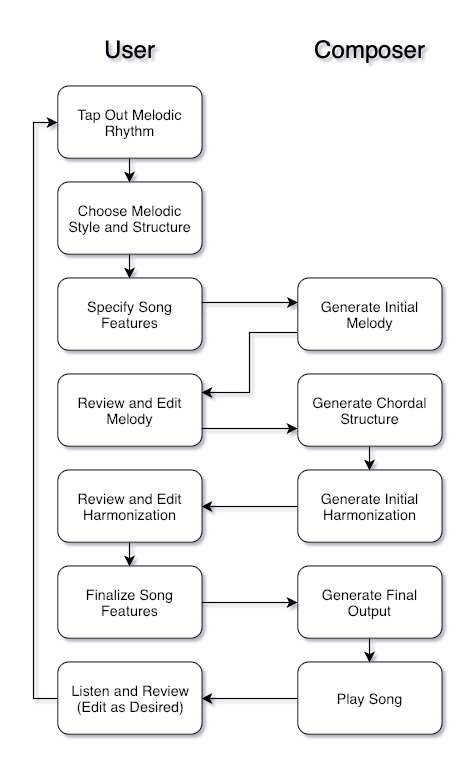
\includegraphics[scale=0.7]{images/composerProcess.png}
\end{figure}

\pagebreak

\subsubsection{Melody Generation}
\label{subsubsec:melody}

During this initial part of the composition process, the computer assists the user in creating a "good" melody.  This involves determining the contour, rhythm, conjunction and disjunctions, and pitches of the melody.  After the melody is generated, the computer determines if it is able to harmonize the melody.  If it is not, it goes back and guide the user through the problematic areas.

\vspace{\baselineskip}

The user also has the opportunity to change the melody if they do not like the way that it sounds or are not satisfied with what they have created.  The computer also provides tips on how to make better melodies and makes suggestions based on the melody that has been generated.

\subsubsection{Harmonization}
\label{subsubsec:harmony}

Next, the computer takes the melody that it has determined that it can harmonize and performs an initial harmonization.  By default, this follows the standard progression of chords in western music as displayed below.

\begin{figure}[h!]
	\centering
	\caption{Standard major key harmonic progression}
	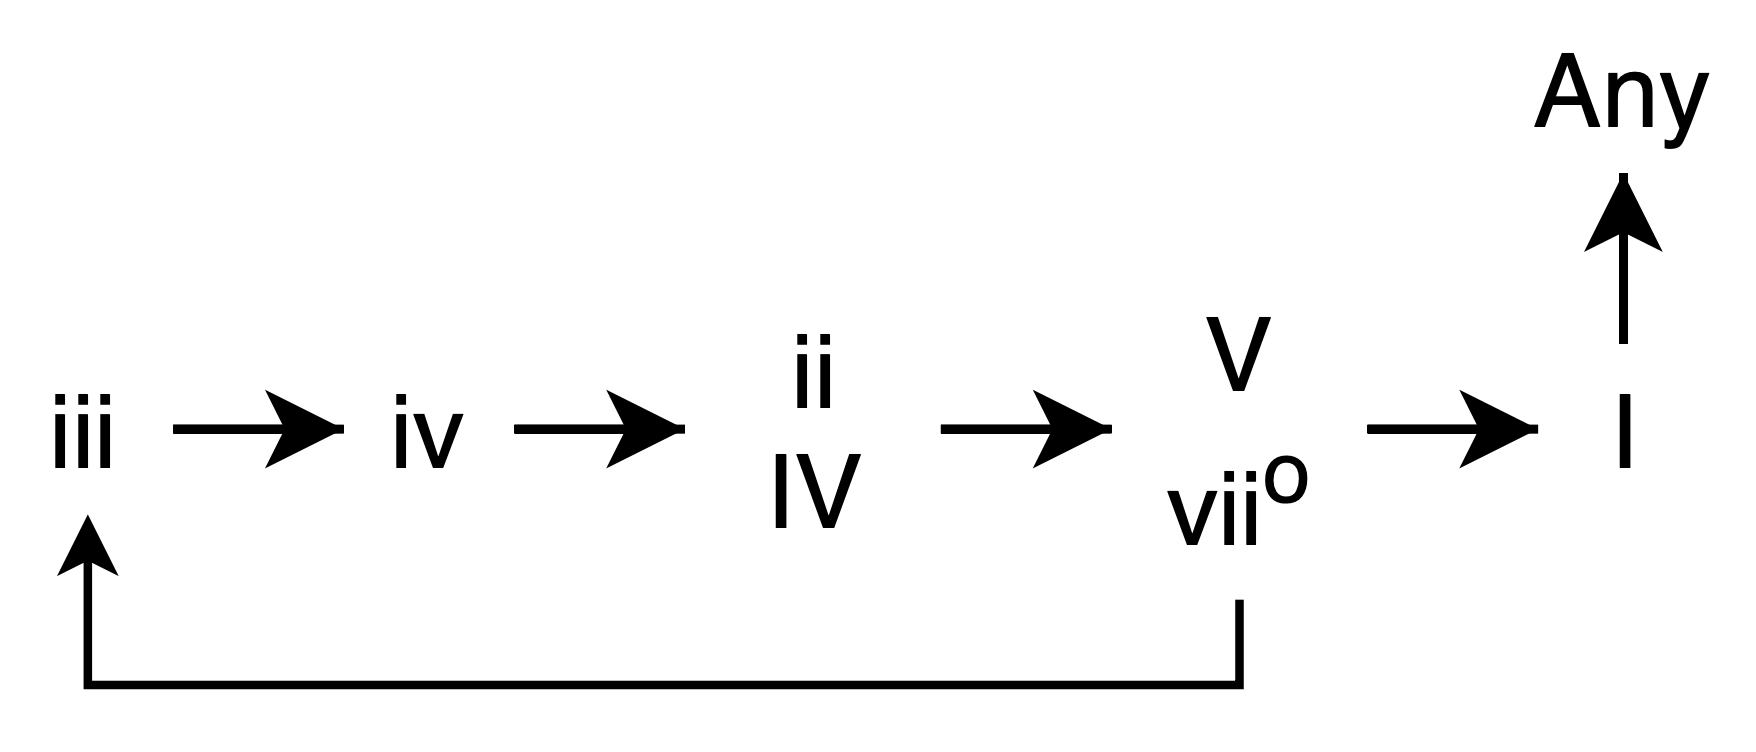
\includegraphics[scale=0.25]{images/majorProgression.png}
\end{figure}

\begin{figure}[h!]
	\centering
	\caption{Standard minor key harmonic progression}
	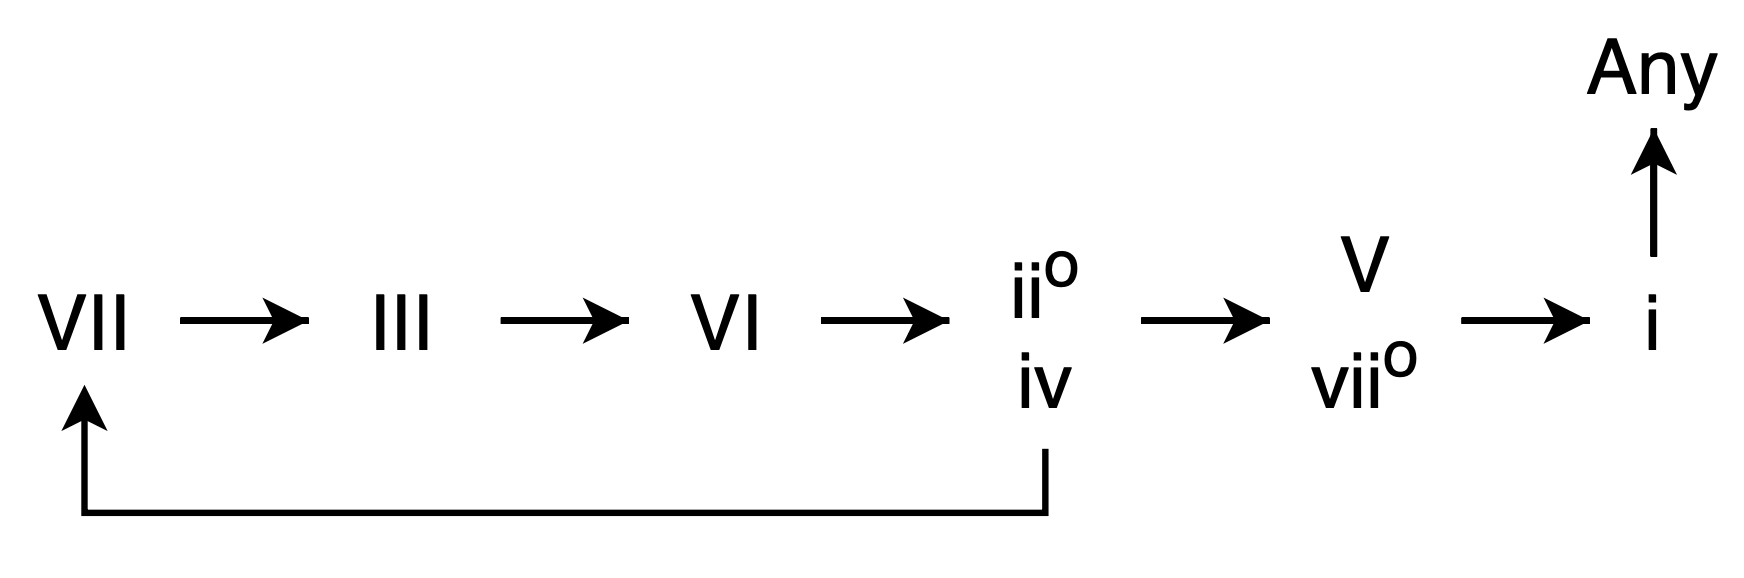
\includegraphics[scale=0.33]{images/minorProgression.png}
\end{figure}

The user is presented with a listing of the chords created during the harmonization and has a change to hear the progression and choose an alternative chord that still fits the melody.  The user also has the option to create their own progression without the rules of western progression in place.

\subsubsection{Key and Metric Analysis}
\label{subsubsec:analysis}

The next step in the composition process metric and key analysis of the melody and harmony that were previously generated.  This step is important for adding additional parts during orchestration and the final notation step.  For the purpose of sound to the user, this does not matter, but it is require to be able to notate the composition.

\vspace{\baselineskip}

This step also contains mood analysis for the purpose of providing the user with an idea of how what they are composing might feel.  This provides them with a general affect of the piece and gives them some information as to what sound set of instruments to pick from.

\subsubsection{Orchestration}
\label{subsubsec:orchestration}

During this step of the process, two things occur.  The user is given the option to generate additional parts such as other accompaniment tracks or percussion and they are presented with the selection of sounds to assign to each of the parts and voices.  All of these choices can be revised or changed later.

\subsubsection{Notation}
\label{subsubsec:notation}

Now that everything has been created and all the parts have been generated, the MIDI data is translated into printable notation files that can be used for the performance and sharing of the composition.  The user can also take the MIDI file generated and put it in another program to perform deeper or more intensive edits or to have access to a different set of sounds for playback.

\subsection{Tools}
\label{subsec:tools}

The following is a descriptive list of the tools that were used in the creation of this composer.

\begin{itemize}
	\item MIDI Miner
	\begin{itemize}
		\item This is a Python library that is capable of analyzing music's tonal tension and classifying parts into different musical segments.  This is used in the composition process to determine the mood and structure of the musical output.
	\end{itemize}
	\item MIDI Musical Accompaniment
	\begin{itemize}
		\item This is a tool, written in Python, that creates musical accompaniment after being provided with instructions in a text file.  This tool is used to generate additional parts automatically based on the lines that the user creates.  The instruction file is be populated by user choices such as style and tempo and by the composer's analysis with details such as key and structure.
	\end{itemize}
	\item Kodou
	\begin{itemize}
		\item Kodou is a Python package that does algorithmic music notation.  This was helpful to be able to take the music created by the tool and output it to a file in standard music notation so that it can be taken and read by another musician.
	\end{itemize}
	\item mingus
	\begin{itemize}
		\item This is a tool that is capable of a number of useful functions for this composer.  Generally, it is a music theory and notation package for Python, but more specifically, it can help build editors, educational music theory tools, and other music processing applications.
	\end{itemize}
	\item LilyPond
	\begin{itemize}
		\item LilyPond Is a program that can interface with a Python program in order to output music notation files.  Kodou and mingus both use LilyPond for their notation output functions.
	\end{itemize}
	\item music21
	\begin{itemize}
		\item This is a set of tools that was developed by MIT for music theory, music computation, and generative composition.  music21 contains the central set of functions that power the composer.
	\end{itemize}
	\item Improviser
	\begin{itemize}
		\item This is Python based software that was created to perform real-time music generation.  Improviser is used in conjunction with music21 to perform the bulk of the back-end work when generating the compositions.
	\end{itemize}
\end{itemize}